\documentclass[12pt, a4paper]{article}
\usepackage[margin=2.0cm]{geometry}
\usepackage{stmaryrd}
\usepackage{amsmath}
\usepackage{amssymb}
\usepackage{enumerate}
\usepackage{bbold}
\usepackage{dsfont}
\usepackage{algorithm2e}
\usepackage{changepage}
\usepackage{undertilde}
\usepackage{hyperref}
\hypersetup{pdftex,colorlinks=true,allcolors=blue}
\usepackage{hypcap}
\usepackage{fancyhdr}
\usepackage{float}
\usepackage[english]{babel}
\usepackage{graphicx}
\usepackage{caption}
\usepackage{subcaption}
\usepackage{wrapfig}
\usepackage{multicol}

\pagestyle{fancy}
\fancyhf{}
\lhead{dc14770}
\rhead{HPC CW2}

\setlength{\parskip}{.1in}
\setlength{\parindent}{0in}
\setlength{\columnsep}{0.5cm}

\begin{document}

  \vspace{.1in}
	\begin{center}
	{ \Large High Performance Computing }

  \end{center}
  \begin{center}

  Coursework 3 Report

	Dylan Cope (dc14770)

	\vspace{.1in}

	\end{center}

  \section*{Introduction}

  Starting with the serial optimisations performed in the first coursework, this report outlines the optimisations made using OpenCL to parallelise the program. For this coursework the Lattice-Boltzmann algorithm was run on four 2D grids of sizes 128x128, 128x256, 256x256 and 1024x1024 to analyse how the optimisations are effected by scaling. The baseline runtimes for these inputs are 105, 213, 855 and 3477 seconds respectively, any optimisations will be measured as speed ups from these times.

  \section*{Basic OpenCL Kernels and Reduction}

  \begin{multicols}{2}

    From the provided base OpenCL code that had implemented kernels for the accelerate flow and propagate functions, the natural next step was to set up kernels for the remaining functions; rebound, collide and average velocity. The rebound and collide functions contained code that iterated across the grid and updated the cells array using the corresponding value in the temporary cells array. This meant the conversion to an OpenCL kernel was as simple as copying the loop functionality into kernels, these kernels were then enqueued with each work item dealling with a coordinate of the grid.

    The average velocity function wasn't so simple to parallelise because of the accumulation of total velocity and total cells. The first step was in noticing the total cells value is constant throughout the entire program, hence it was computed before the time steps and the average velocity function was replaced with a total velocity one. Now the problem was a simpler reduction of velocities across the cells array.

    This reduction was implemented by creating a kernel for which each work group was designed to summate velocities of a contiguous section of the cells array. Table \ref{reduproc} outlines this process.
  \end{multicols}

  \begin{table}[ht!]
    \centering
    \vspace{-0.5cm}
    \caption{Total velocity reduction process}
    \label{reduproc}
    \begin{tabular}{lllllllllll}
        &                              &                              & $| \leftarrow$                  & $\dots$                      &                                 & work group $i$                  &                                 & $\dots$                      & $\rightarrow |$                 &         \\ \cline{3-11}
    (1) &                              & \multicolumn{1}{l|}{$\dots$} & \multicolumn{1}{l|}{$t\_speed$} & \multicolumn{1}{l|}{$\dots$} & \multicolumn{1}{l|}{$t\_speed$} & \multicolumn{1}{l|}{$t\_speed$} & \multicolumn{1}{l|}{$t\_speed$} & \multicolumn{1}{l|}{$\dots$} & \multicolumn{1}{l|}{$t\_speed$} & $\dots$ \\ \cline{3-11}
    (2) &                              &                              & $\downarrow$                    & $\downarrow$                 & $\downarrow$                    & $\downarrow$                    & $\downarrow$                    & $\downarrow$                 & $\downarrow$                    &         \\ \cline{4-10}
     &                              & \multicolumn{1}{l|}{}        & \multicolumn{1}{l|}{$float$}    & \multicolumn{1}{l|}{$\dots$} & \multicolumn{1}{l|}{$float$}    & \multicolumn{1}{l|}{$float$}    & \multicolumn{1}{l|}{$float$}    & \multicolumn{1}{l|}{$\dots$} & \multicolumn{1}{l|}{$float$}    &         \\ \cline{4-10}
    (3) &                              & $v_t \leftarrow $                        & $+\hookleftarrow$               & $+\hookleftarrow$            & $+\hookleftarrow$               & $+\hookleftarrow$               & $+\hookleftarrow$               & $+\hookleftarrow$            & $+\hookleftarrow$               &         \\
    (4) &                              & $\downarrow$                 &                                 &                              &                                 &                                 &                                 &                              &                                 &         \\ \cline{2-4}
     & \multicolumn{1}{l|}{$\dots$} & \multicolumn{1}{l|}{$float$} & $\dots$                         &                              &                                 &                                 &                                 &                              &                                 &         \\ \cline{2-4}
    \end{tabular}
  \end{table}
  \vspace{-.5cm}
  \begin{itemize}
    \setlength\itemsep{0.0cm}
    \item [(1)] Each work group is given a portion of the global cells to find the total velocity for.
    \item [(2)] Work items in the group compute the velocity for a given cell and place the value in an array local to the work group.
    \item [(3)] Once all the items have placed their values in the local array, the zeroth worker of the group adds together all the values.
    \item [(4)] This partial sum for the global problem is placed in an array to be read back by the host.
  \end{itemize}

  \begin{multicols}{2}

    Once all the work groups finish computing their partial sums the host reads back the array they've written to and adds together the values in it to produce the final total velocity value. The method now begs the questions of how many work groups to implement and how large of a section of the cells array to allocate to each group. By creating the relationship that says the number of work groups is equal to the number of cells divided by a given work group size we can reduce this to asking what the most optimal work group size is.

    Figure \ref{wgs} varies the work group size and plots the corresponding speed up from the baseline runtime values. The graph shows that the optimal region is between 32 and 128 cells per group, before and after that the performance decreases. Its also clear that the improvement doesn't provide any scaling benefit, i.e. the speed up for different grid sizes is roughly equal.

    \begin{figure}[H]
      \caption{} \label{wgs}
      \vspace{-0.8cm}
      \begin{center}
        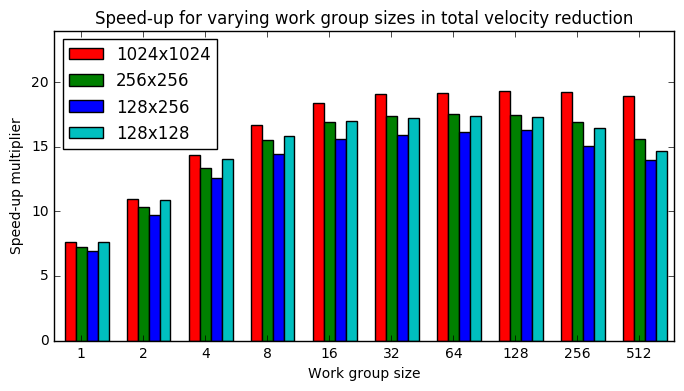
\includegraphics[width=0.5\textwidth]{figures/workgroupsize}
      \end{center}
    \end{figure}


  \end{multicols}

  \section*{Array of Structures to Structure of Arrays}

  \begin{table}[ht!]
  \centering
  \vspace{-.4cm}
  \caption{Varying layouts between paradigms}
  \vspace{-.2cm}
  \label{datalayouts}
  \begin{tabular}{lllllllll}
                                &                              &                              &                              & AoS                          &                              &                              &                              &         \\ \hline
  \multicolumn{1}{l|}{$\dots$}  & \multicolumn{1}{l|}{padding} & \multicolumn{1}{l|}{speed 0} & \multicolumn{1}{l|}{speed 1} & \multicolumn{1}{l|}{$\dots$} & \multicolumn{1}{l|}{speed 8} & \multicolumn{1}{l|}{padding} & \multicolumn{1}{l|}{speed 0} & $\dots$ \\ \hline
                                &                              &                              &                              &                              &                              &                              &                              &         \\
                                &                              &                              &                              & SoA                          &                              &                              &                              &         \\ \hline
  \multicolumn{1}{|l|}{speed 0} & \multicolumn{1}{l|}{speed 0} & \multicolumn{1}{l|}{$\dots$} & \multicolumn{1}{l|}{speed 0} & \multicolumn{1}{l|}{speed 1} & \multicolumn{1}{l|}{$\dots$} & \multicolumn{1}{l|}{speed 1} & \multicolumn{1}{l|}{speed 2} & $\dots$ \\ \hline
                                &                              &                              &                              &                              &                              &                              &                              &
  \end{tabular}
  \end{table}
  \vspace{-.6cm}

  \begin{multicols}{2}

    The base code arranges the cell data as an array of $t\_speed$ structures, where each $t\_speed$ consists of nine values, this is a Array of Structures (AoS) paradigm for arranging a sequence of records in memory. An alternative arrangement is the Structure of Arrays (SoA) paradigm, for which the motivation for using is utilising Same Instruction Mulitple Data (SIMD) architecture. As the NVIDIA GPUs on Blue Crystal that this project is run on support these kinds of operations it makes sense to convert the cell arrays to this form.

    Table \ref{datalayouts} shows the differing layouts for the speed values of the cells arrays. For a process such as $\sum_i (cell_i.speed0 + cell_i.speed4)$, its clear that for AoS arranging inputs into SIMD operation isn't natural, whereas for SoA the program can load all the contiguous speed 0 values into the first input of a SIMD operation and all the speed 4 values into the second input. This kind of computation is done for every work item when the component velocities of a given cell are computed.

    Figure \ref{aos2soa} shows the speed-up for converting from AoS to SoA form. As show the performance increase is substantial, and the optimisation has caused vast scaling improvements. Prior to the conversion the speed up for all the input sizes was roughly equal, however now the larger inputs have sped up relative to their size.

    \begin{figure}[H]
      \caption{} \label{aos2soa}
      \vspace{-0.8cm}
      \begin{center}
        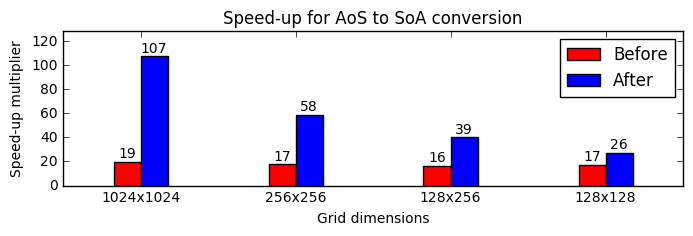
\includegraphics[width=0.5\textwidth]{figures/aos2soa}
      \end{center}
    \end{figure}

  \end{multicols}

  \section*{Kernel Fusing and Branch Masking}

  \begin{multicols}{2}

    At this point in the described optimisations there were four OpenCL kernels; accelerate flow, propagate, rebound and total velocity. The rebound kernel dealt with updating the cells array based on the temporary cells array, the total velocity kernel then iterates over the cells array in a similar fashion.

    Figure \ref{fusekernel} shows the improvement gained from performing these two steps at the same time (i.e. ``fusing'' the two kernels). The difference isn't as hugely significant as the AoS to SoA conversion, but it still clearly has a positive effect on making the program scale better with input size. From this point onward 128 is used as the work group size.

    \begin{figure}[H]
      \vspace{-0.4cm}
      \caption{} \label{fusekernel}
      \vspace{-0.8cm}
      \begin{center}
        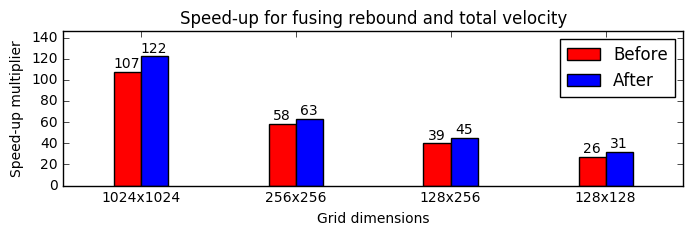
\includegraphics[width=0.5\textwidth]{figures/fusekernel}
      \end{center}
      % \vspace{-0.6cm}
    \end{figure}

    The code in the resultant kernel from the fusing was primarly split into two conditional branches based on if the given coordinate corresponded to an obstacle or not. Considering the situation when multiple cells are loaded into a SIMD operation it's evident how this kind of branching would be a bottleneck - if sections of your contiguous SIMD input need to perform different instructions from one another the only thing to do is to run the instructions serially.

    This is where the techinique of branch masking is used. Rather than performing different instructions based on a condition, the same instruction is run on all the data, however the instruction is a function of the condition. For example if you had a process that sets $v=5$ if $b$ and otherwise $v=3$, this could be masked by replacing the process with $v = 5 \times b + 3 \times !b$.

    Applying this optimisation to the problem resulted in a small improvement, the reason the effect was so small was because of the proportion between obstacle and non-obstacle cells in the input grids. The provided obstacle files have obstacles only around the edge of the grid, and hence approximately 99\% of the grid is free cells. The whole advantage of the branch masking technique was to have more efficient SIMD operations when the input vector has elements that branch in different ways, however for the vast majority of operations all the elements were already branching one way or another.

    This implies the new program should perform better with less extreme obstacle to non-obstacle ratios. An obstacle input file for the 256x256 grid was generated with 50\% of the cells being obstacles, for this input the version with branch masking ran two seconds faster than the one without. On the otherhand the runtime differences between the versions with 10\% or 90\% of the being obstacles was under a second, hence confirming the hypothesis that branch masking makes the program more flexible for dealing with input files.

  \end{multicols}

  \section*{Further Management of the Memory Hierarchy}


\end{document}
